
\chapter{Ocean water masses}
\label{ch:watermasses}


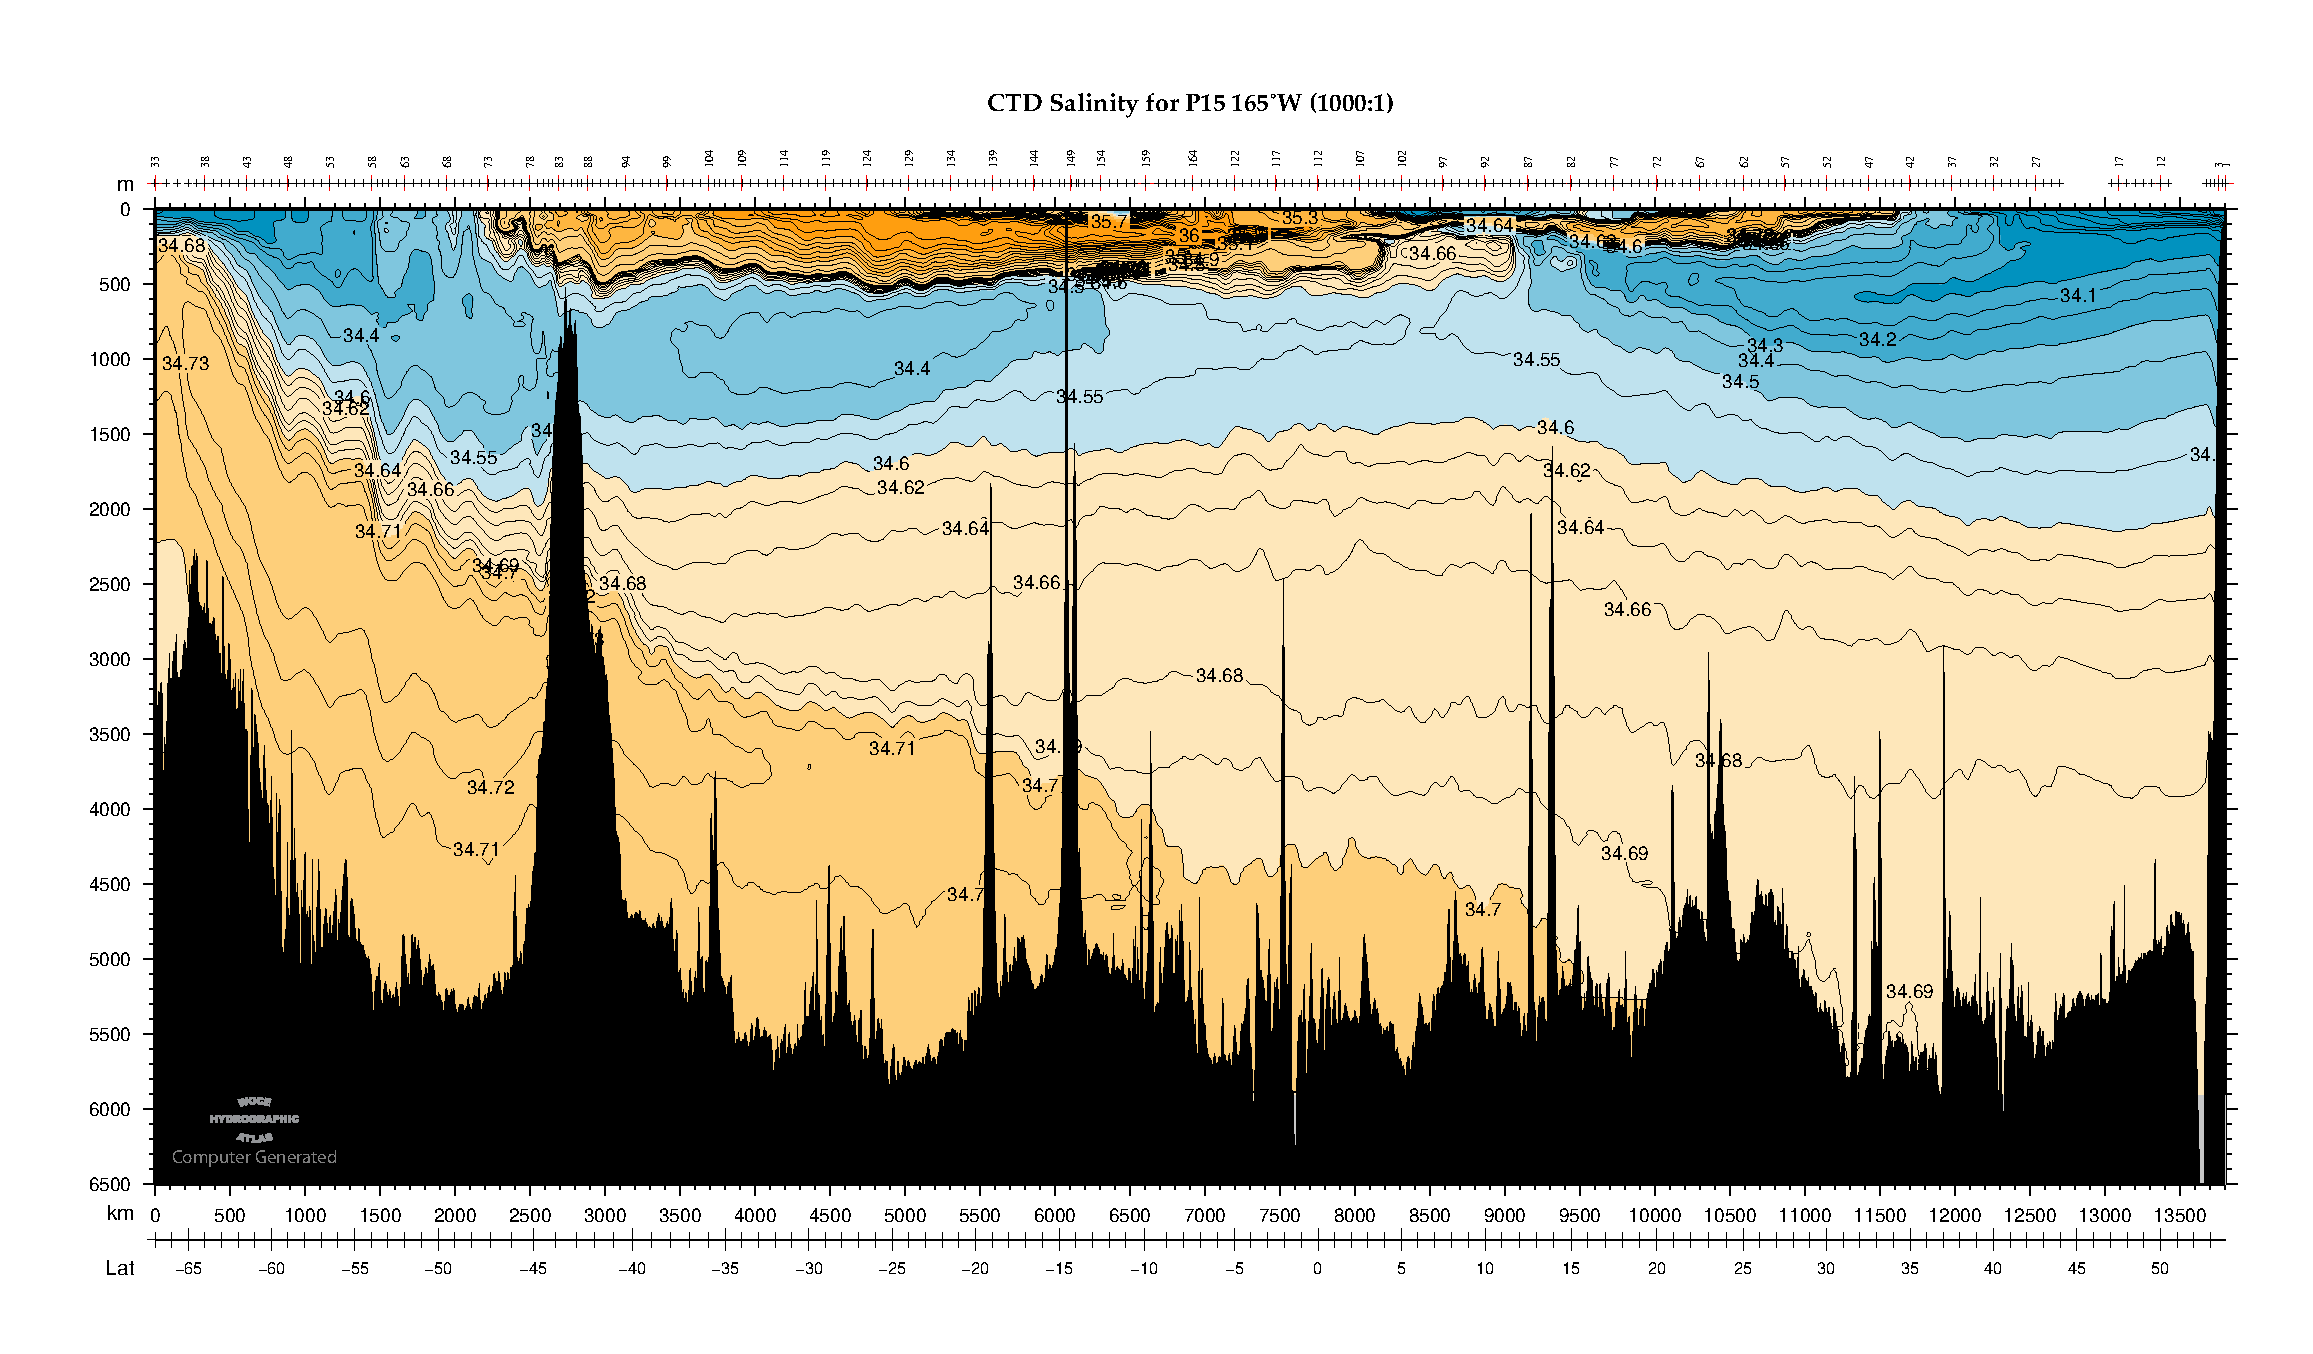
\includegraphics[width=6.5in]{figs/WaterMasses/P15_CTDSAL_all_1000.pdf}


Most exchange of ocean heat and freshwater occur at the surface of the ocean, with only minor contributions due to geothermal heatfluxes, and exchange of solutes with the crust.   Thus water that is ``formed'' at the surface tends to retain its signature as it moves through the ocean, leading to the concept of identifiable ocean water masses.  These water masses are thought of as having ``core'' values of temperature and salinity that then are diluted by mixing with other water masses.  This approach is of course most effective with water masses that are far from the surface of the ocean where they are not modified, so we concern ourselves primarily with \emph{intermediate} and \emph{deep} water masses here.  

\section{Surface distributions of temperature and salinity}

\begin{figure}[hbt]
  \begin{center}
  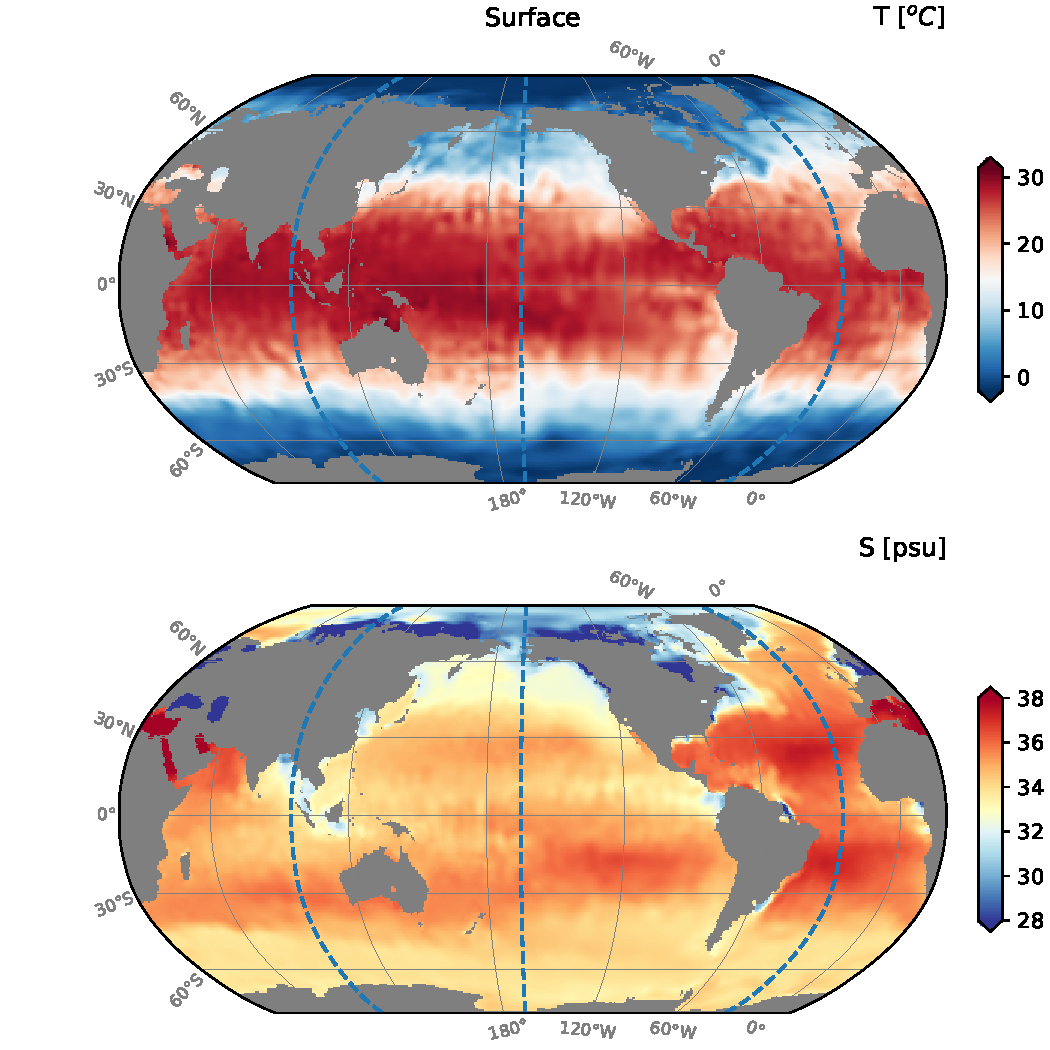
\includegraphics{figs/WaterMasses/SurfaceTS}
    \caption{Annual average surface temperature and salinity from the \href{https://icdc.cen.uni-hamburg.de/en/woce-climatology.html}{WOCE climatology}.  Dashed lines are sections shown below in the Pacific, Atlantic, and Indian Oceans.}  
    \label{fig:SurfaceTS}  
  \end{center}
\end{figure}

Temperature and salinity distributions at the surface of the ocean follow relatively predictable patterns given the fluxes in \fref{ch:heatsaltflux} (\fref{fig:SurfaceTS}).  Warm water is found near the equator, and cold at the poles.  There is a relatively sharp delineation between warm waters and cold waters just poleward of approximately 45 degrees, particularly in the Northern Hemisphere, a signature of the separation of the western boundary currents from the continents (like the Gulf Stream) at those latitudes.   There is often relatively cool water directly adjacent to the western shore of continents due to upwelling.  

Salinity is more complicated with relatively salty surface water at the mid latitdes, and fresher water in the subpolar gyres and the equator.  The Mediterranean, Red Sea, and Persian Gulf are very salty, and overall the Atlantic and Indian oceans are much more salty than the Pacific, to no small part because of these marginal seas.  


\section{Meridional sections}

Clearly the largest variation at the surface of the ocean in temperature and salinity is in the \emph{meridional} direction (North-south), so we start our exploration of the water masses in the ocean by looking along meridians in the Pacific, Atlantic, and Indian oceans (\fref{fig:AllTSSection}).  There are striking similarities between all three basins, particularly in the Southern hemisphere, with the largest differences in the salinity distribution amongst the oceans.  

\begin{figure*}
  \centering
  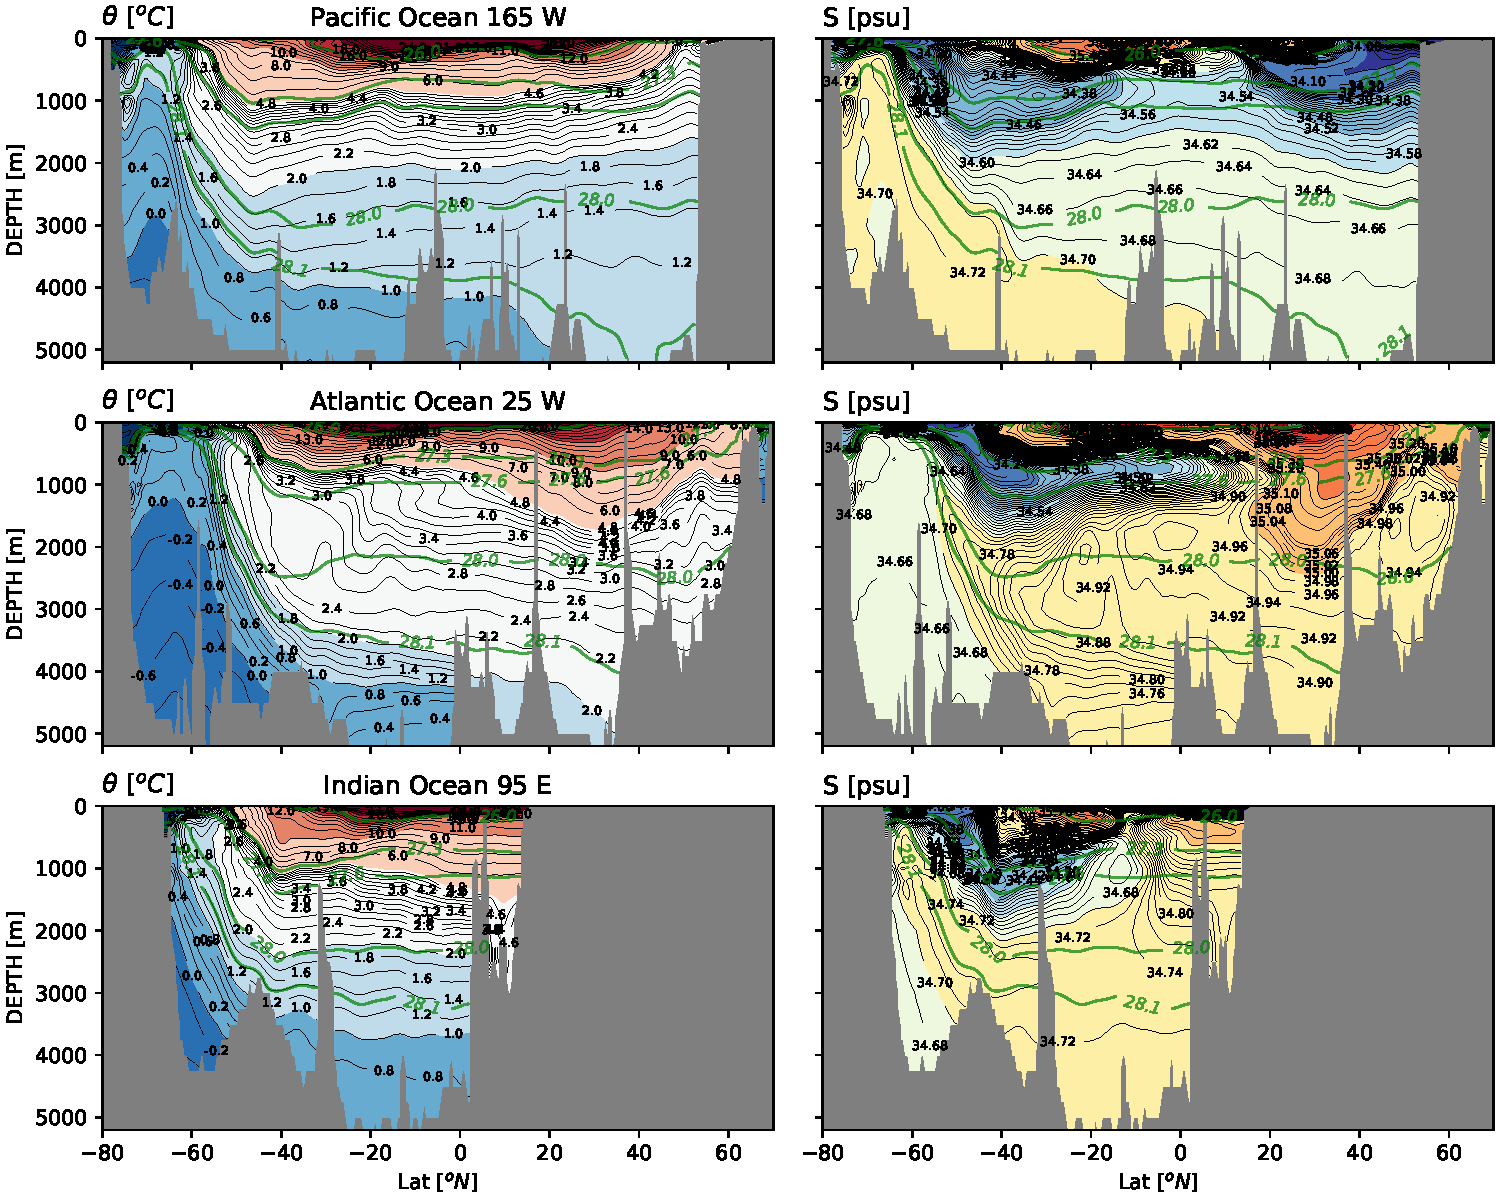
\includegraphics[width=7in]{figs/WaterMasses/AllTSSection}
    \caption{North-south cross sections of potential temperature and salinity in the world's oceans.  Green contours are levels of constant neutral density.  Note the contour levels and colors are non-linear and chosen to highlight ocean water masses. Note the location of these sections is shown in \fref{fig:SurfaceTS}, \fref{fig:TSGammaSurf}, and \fref{fig:TSDepthSurf} }
    \label{fig:AllTSSection}  
\end{figure*}

\paragraph{Surface waters}
First, in the upper ocean, shallower than 700 m or so, there is a distinct push down of both the isotherms and isohalines centered around 30 degrees.  These surfaces rise at the equator, and then again as we move poleward of 30 degrees.  This is the signature of the wind-driven \emph{subtropical gyres}, and will be discussed in later chapters.  These surface waters are characterized by relatively warm, salty water.  Poleward of these bowls are the \emph{subpolar gyres} which tend to be cooler and significantly fresher.  

\begin{figure*}
  \centering
  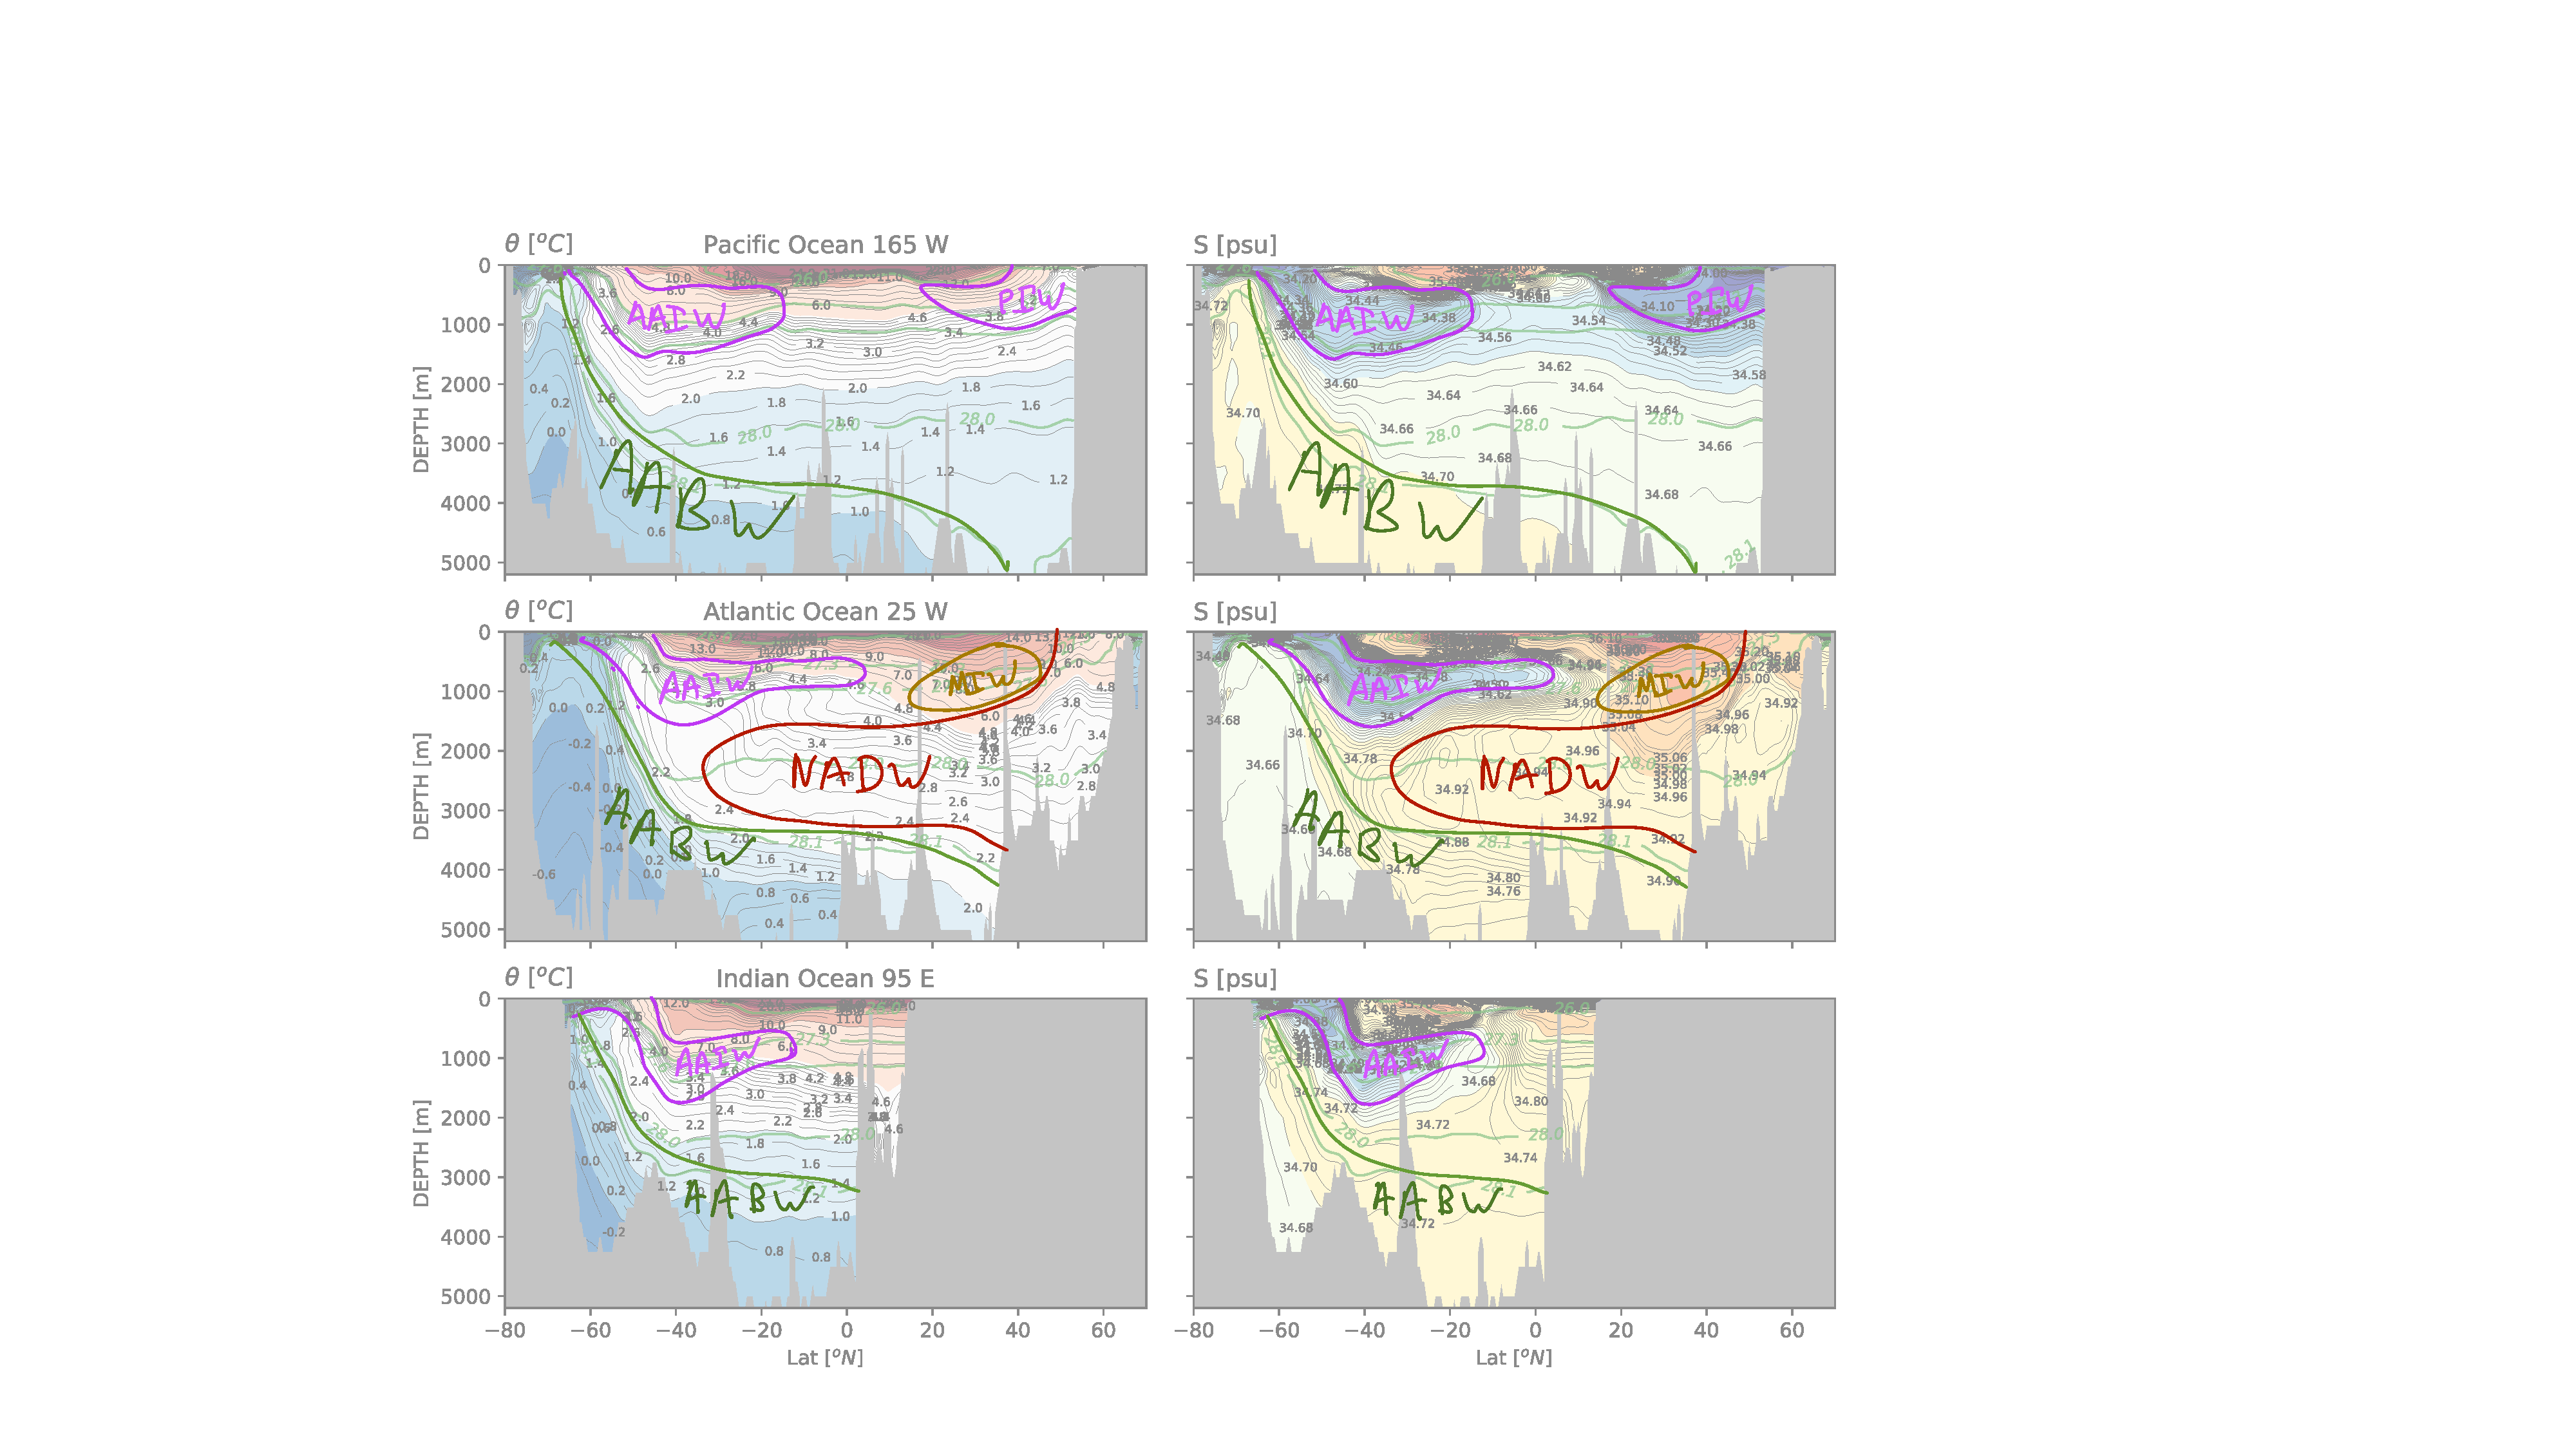
\includegraphics[width=7in]{figs/WaterMasses/AnnotateSections}
    \caption{As in \fref{fig:AllTSSection}, with intermediate and deep water masses indicated.  AAIW: Antarctic Intermediate Water, PIW: Pacific Intermediate Water, MIW: Mediterranean Intermediate Water, ABW: Antarctic Bottom Water, NADW: North Atlantic Deep Water}
    \label{fig:AnnotateSections}  
\end{figure*}


\paragraph{Intermediate waters} Below the surface water, at depths approximately 1000 m are the Intermediate waters.  There is a tongue of fresh cool water found at this depth in all the oceans, clearly connected to the sub-polar gyre in the Southern Ocean, so this water is called \emph{Antarctic Intermediate Water}.  This water is found in all the ocean basins as a northward protruding tongue of water pushed down at around 50 S and then moving up slightly as it moves north (\fref{fig:AnnotateSections}: AAIW).  An analogous water mass is found in the North Pacific, and is usually called North-Pacific Intermediate water (\fref{fig:AnnotateSections}: PIW) which originates near 50 N and then is pushed south under the subtropical gyre water.  

Finally, there is the very distinct intermediate water mass found in the North Atlantic, called \emph{Mediterranean Intermediate Water} (\fref{fig:AnnotateSections}: MIW).  This very salty water is formed in the Mediterranean where salinities exceed 38 psu, which then pours into the North Atlantic as dense water.  This water mixes with the ambient water and is diluted, but still has a very robust salinity structure that is found throughout the North Atlantic at the intermediate depths.

\paragraph{Deep and bottom waters} Finally, all basins have water along the bottom composed of the densest water in the ocean.  Its clear from these cross sections that this water originates in the Southern Ocean (\fref{fig:AnnotateSections}:AABW), where it can be seen \emph{outcropping} south of 60 S, and therefore we call this \emph{Antarctic Bottom Water}.  We have the distinct impression that it moves north, as we would expect from the slope of the density surface, and that it becomes diluted with the fresher and warmer above as it moves further north.  

The last major water mass is \emph{North Atlantic Deep Water} (\fref{fig:AnnotateSections}: NADW).  This water is produced in the Greenland-Iceland Seas, and to a lesser extent the Labrador Sea, and is not as dense as Antarctic Bottom Water.  Its density is centred around $\gamma_N \approx 28$, and flows into the ocean above the AABW from the north to the south.  

There are many ways to look at these water masses in addition to meridional sections.  Surfaces of constant depth (\fref{fig:TSDepthSurf}) and surfaces of constant neutral density (\fref{fig:TSGammaSurf}) give a useful reference as to where the water masses come from.  For instance the Mediterranean water is very clear at $Z=2000\ \mathrm{m}$ (\fref{fig:TSDepthSurf}) as a tongue of salty water.  Its also warmer, as can be seen in the contours of temperature, but it is not as obvious due to the colormap.  We can see that the fresh intermediate water clearly at $1000\ \mathrm{m}$ in the North Pacific is fresher on the west side of the basin than the east.  

The deepest surfaces ($Z = 4000 \ \mathrm{m}$) are interesting in that we can see cold salty water pouring in the Pacific (\fref{fig:TSDepthSurf}).  We note that it preferentially flows in on the west side of the basin, which is due to the Coriolis force turning the flow to the left.  This can be seen, somewhat less dramatically, in the other basins.  A similar effect happens with the North Atlantic Deep Water, where it flows south, it hugs the western boundary (because it is turning to the right due to the Coriolis force) though it is less obvious to see in these plots.  

\begin{figure*}
  \centering
  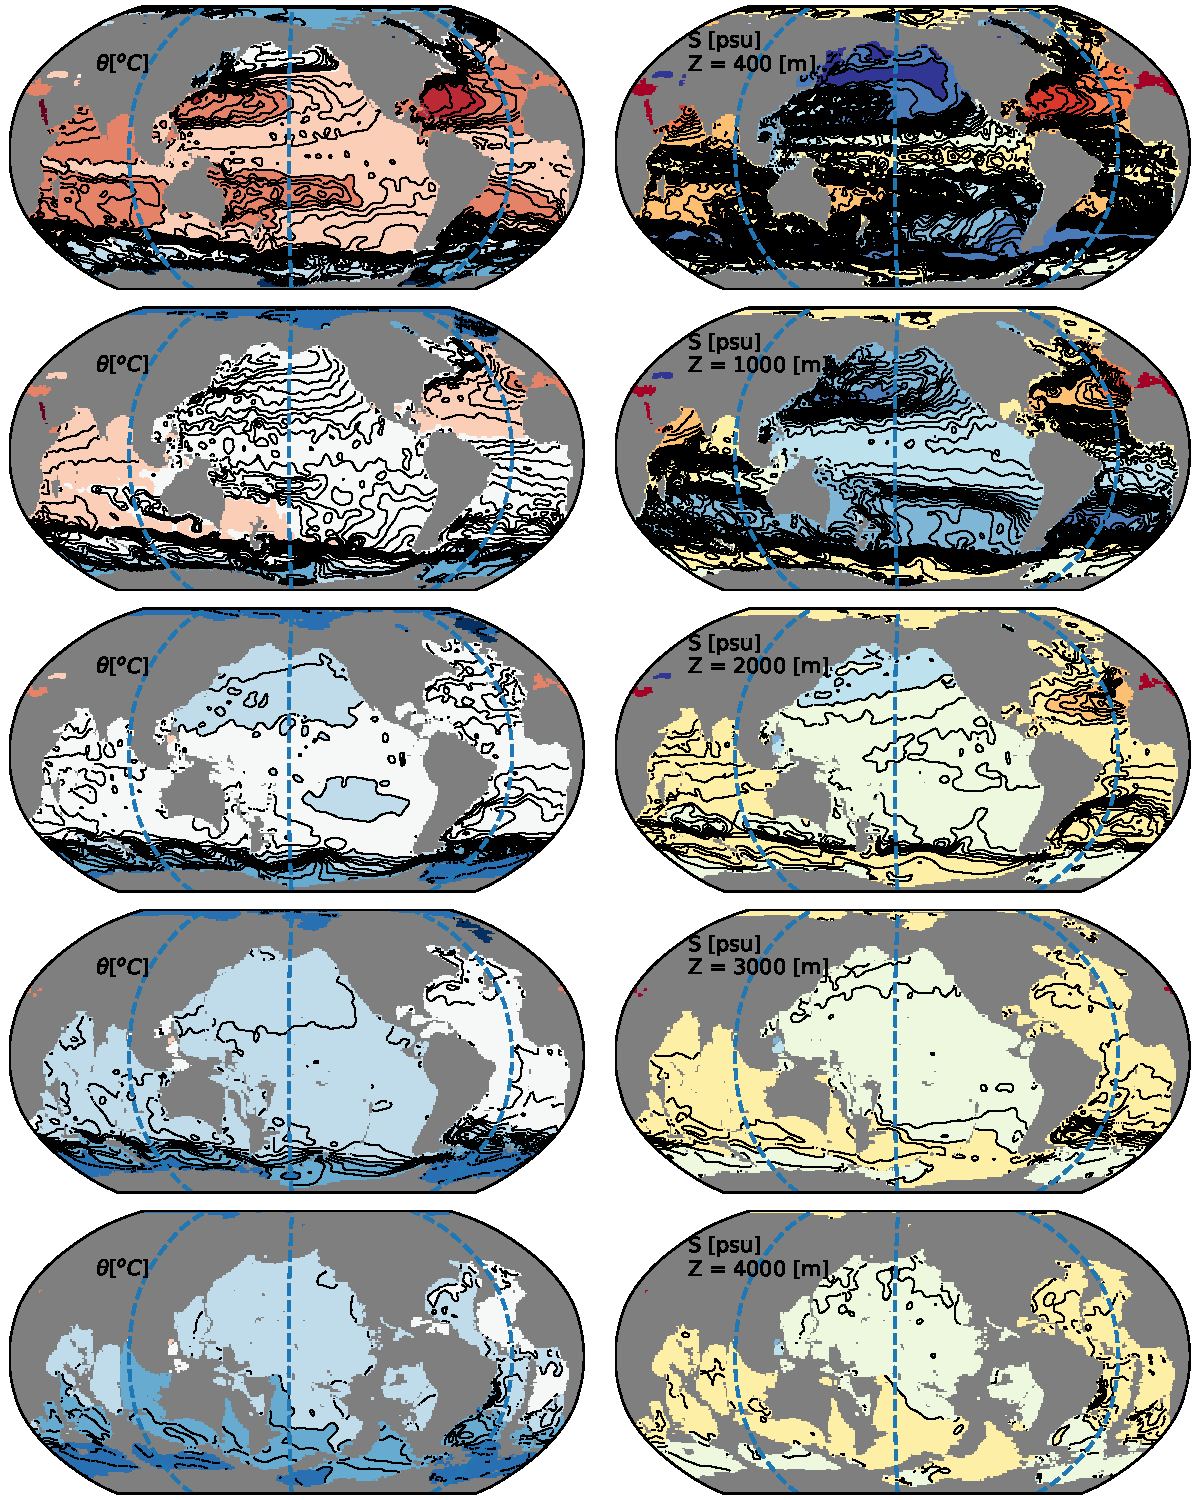
\includegraphics[width=7in]{figs/WaterMasses/TSDepthSurf.pdf}
    \caption{Global views of potential temperature and salinity on surfaces of constant depth.  Dashed blue lines are sections shown in \fref{fig:AllTSSection}}
    \label{fig:TSDepthSurf}  
\end{figure*}

\begin{figure*}
  \centering
  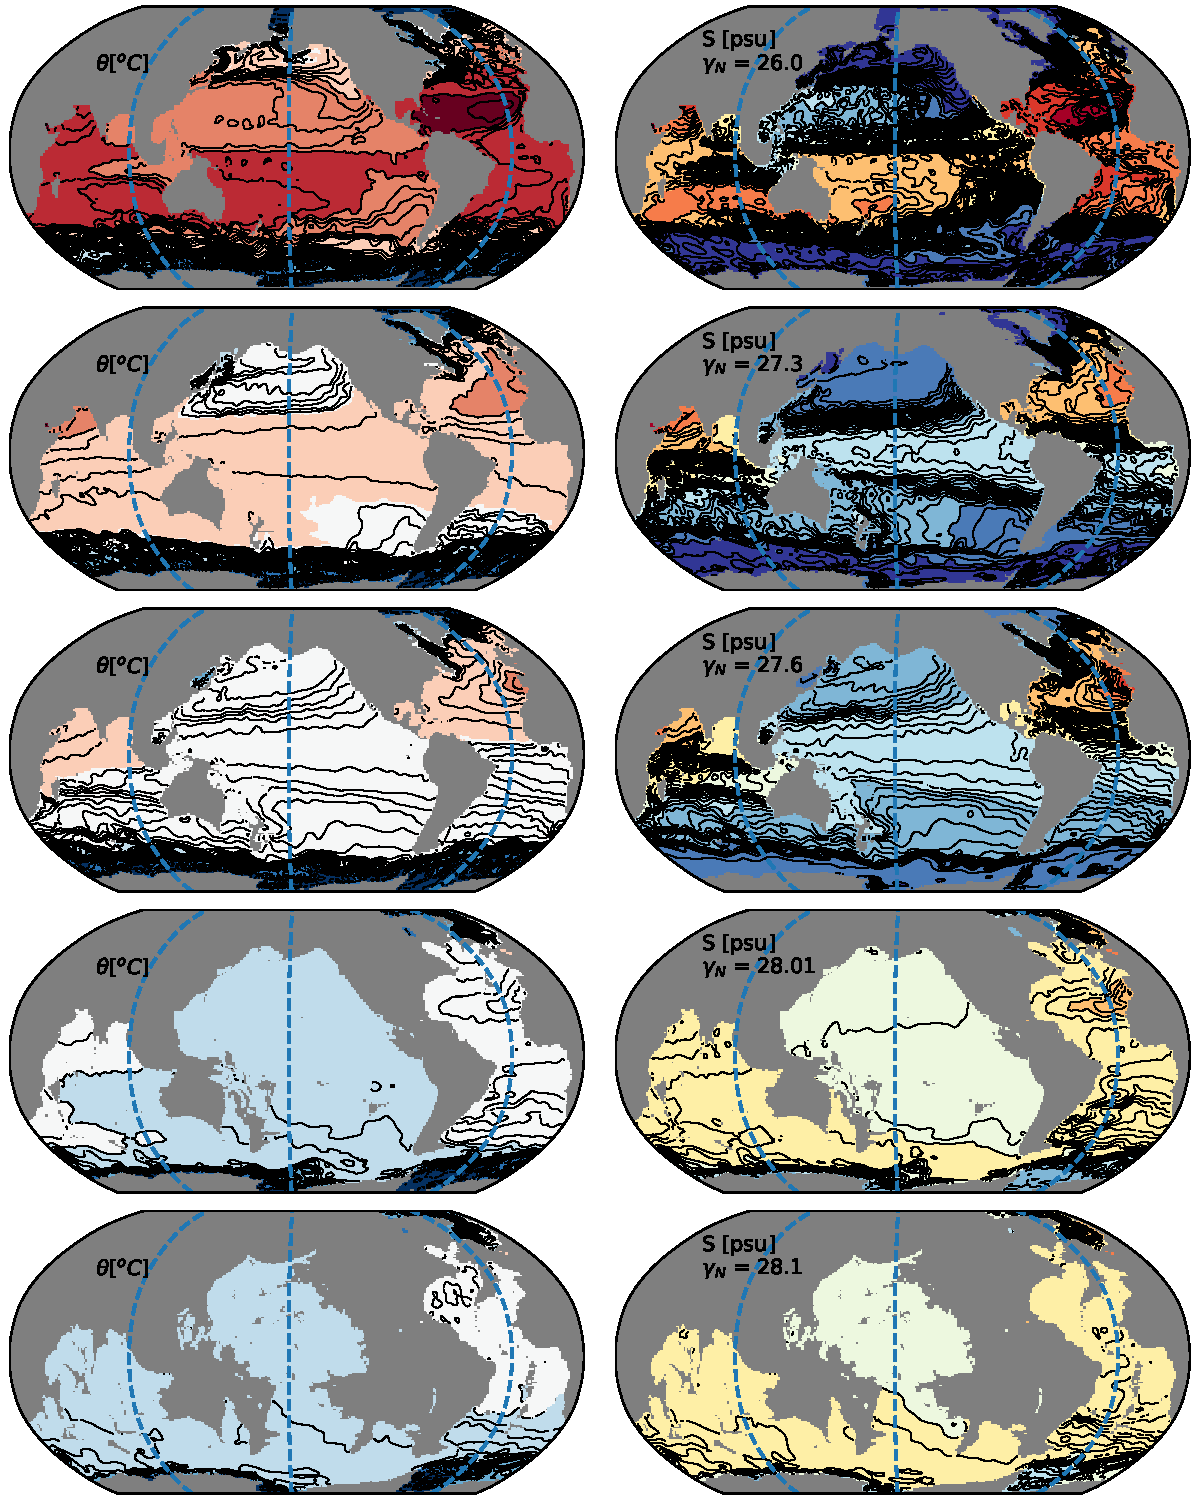
\includegraphics[width=7in]{figs/WaterMasses/TSGammaSurf.pdf}
    \caption{Global views of potential temperature and salinity on neutral density surfaces.  The surfaces chosen are the same ones contoured in \fref{fig:AllTSSection} in green.   Dashed blue lines are sections shown in \fref{fig:AllTSSection}}
    \label{fig:TSGammaSurf}  
\end{figure*}

Overall these plots reinforce the idea that most of the variation is in the meridional direction, with details showing up in the zonal direction.  These east-west differences tend to be most pronounced near the coasts, or adjacent to marginal seas like the Mediterranean.  

\section{Vertical distributions, and the surface mixed layer}

It is worth re-iterating that the plots made above have very non-linear colormaps, and that most of the ocean's variability is in the upper ocean (\fref{fig:ExamplePacificProfiles}) with weak, but very consistent, gradients at depth.  This structure applies through much of the ocean with most of the variation taking place across a \emph{thermocline} that is on the order of 1000 m thick, decaying into a relatively homogeneous abyss for the rest of the ocean.  

\begin{figure*}
  \centering
  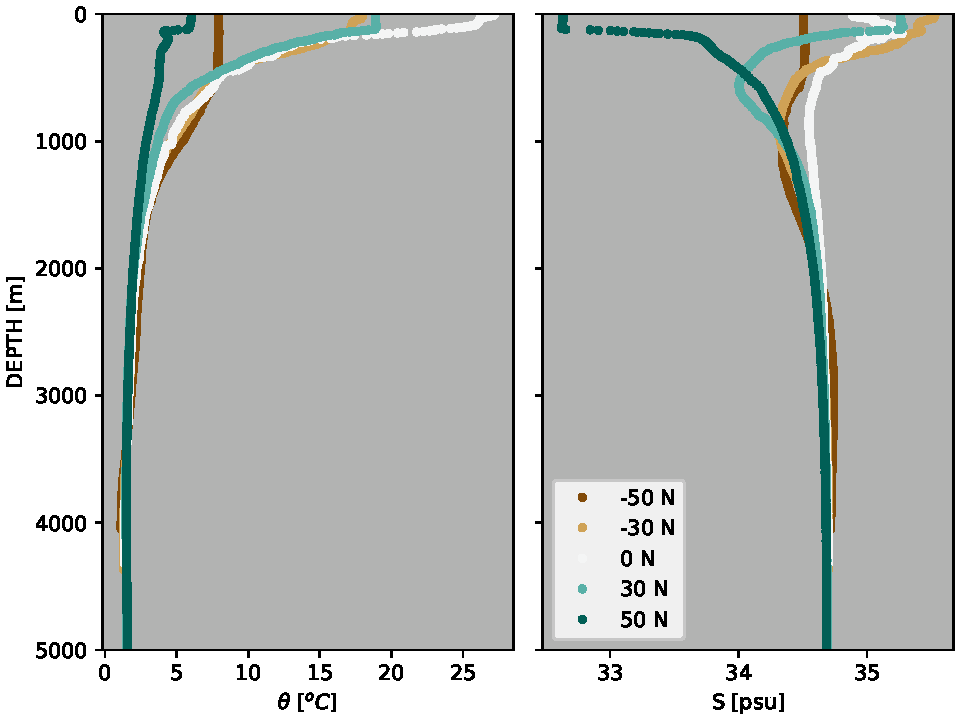
\includegraphics[width=3in]{figs/WaterMasses/ExamplePacificProfiles}
  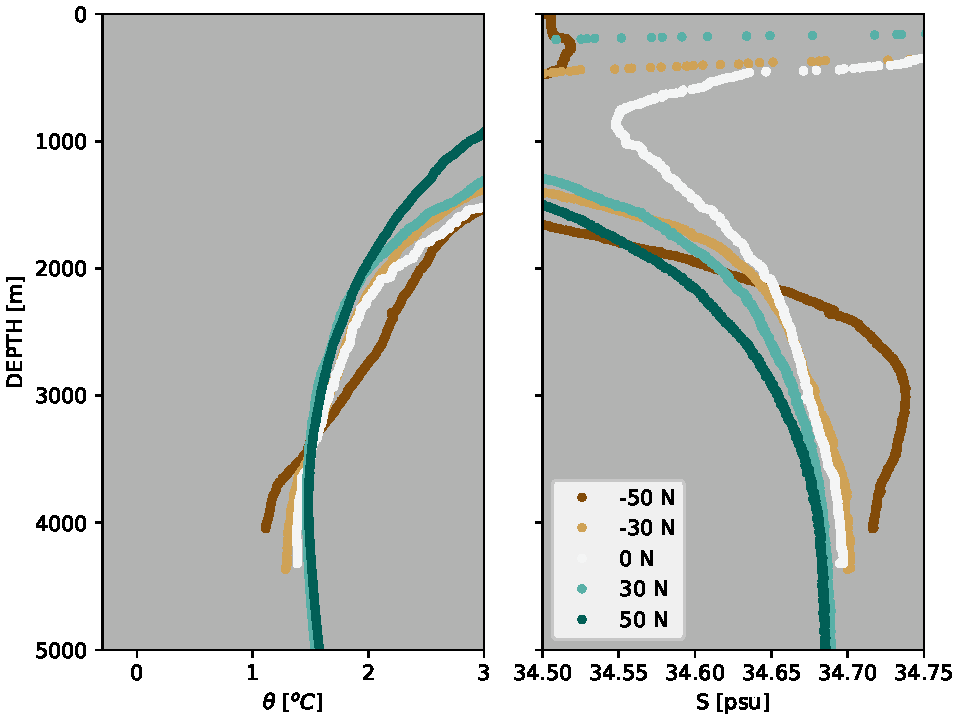
\includegraphics[width=3in]{figs/WaterMasses/ExamplePacificProfilesZoom}
    \caption{Example $\theta$ and $S$ profiles from the Pacific Ocean at five different latitudes.  The two plots on the right as zoomed version of the plots on the left.  }
    \label{fig:ExamplePacificProfiles}  
\end{figure*}

The upper ocean is usually topped by a \emph{mixed layer}, where the action of waves and wind have combined to mix the water uniformly.  This can be seen in all the example profiles in \fref{fig:UpperPacProfile}, except for the profile at the equator (white) as a region of homogeneous water in both the temperature and salinity profiles.  At 50 S, this layer is particularly thick, extending over 150 m deep.  In the plot shown it looks like it is much deeper, but there is some slight temperature and salinity difference with depth that stops the water from being completely homogeneous.

\begin{figure}[htp]
  \centering
  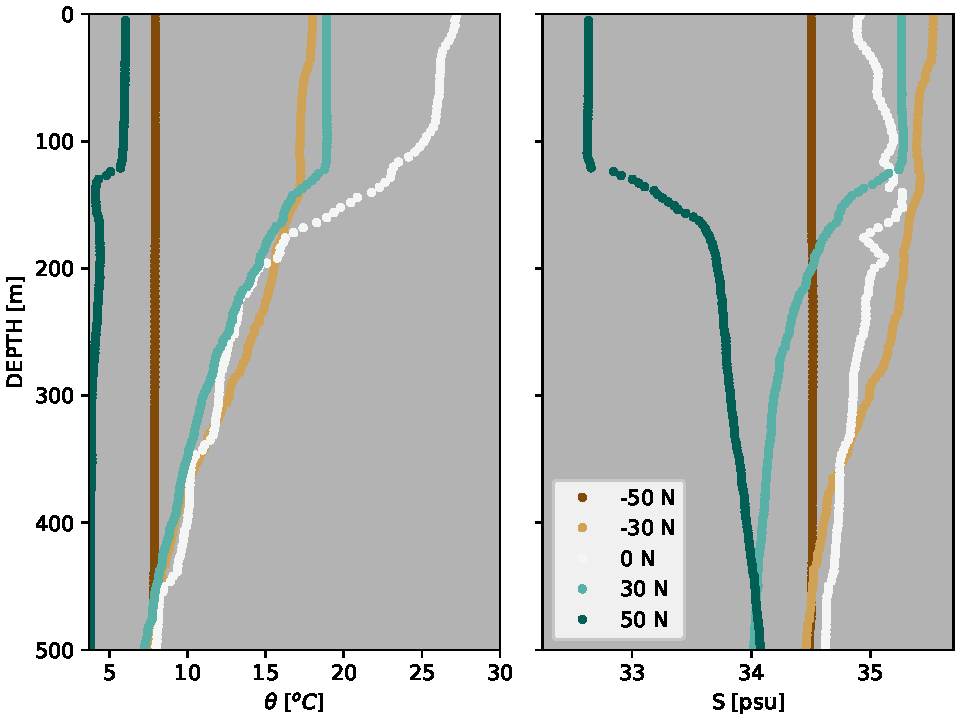
\includegraphics[width=3in]{figs/WaterMasses/UpperPacProfile}
    \caption{Example $\theta$ and $S$ profiles from the Pacific Ocean at five different latitudes.  The two plots on the right as zoomed version of the plots on the left.  }
    \label{fig:UpperPacProfile}  
\end{figure}

The dynamics of the mixed layer are very important given that they mediate the flux of temperature and gasses between the ocean and the atmosphere.  There are three things that deepen the mixed layer:
\begin{enumerate}
    \item Cooling from evaporation and sensible heat loss
    \item Mixing from wind-driven turbulence and waves
    \item Shear-driven turbulence at the base of the mixed layer.
\end{enumerate}
The first term is relatively straight forward.  The second term is hard to parameterize, but accords with  our usual understanding of waves as turbulent forces.  The last term is because the wind pushes the mixed layer, and hence it develops momentum that is different in speed and direction from the water below.  This generates a \emph{shear} and these can go unstable (\fref{ch:mixing}).  

The mixed layer will \emph{restratify} due to 
\begin{enumerate}
    \item Heating or freshwater
    \item Lateral advection of more buoyant water (often from equatorward).  
\end{enumerate}

This cycle leads to an annual/seasonal cycle of the upper ocean mixed layer (\fref{fig:PellandEtAl}), with cooling in the winter, and warming in the summer.  In this case, the mixed layer gets down to about 100 m by later spring, and then starts shoaling again in the summer.  This often leads to a situation where there are two thermoclines in the summer; the \emph{permanent thermocline} deeper than 100 m, and a \emph{seasonal thermocline} beneath the summer mixed layer.  Note that in this example, the mixed layer is also strongly influenced by salinity, so the concept of the \emph{halocline} is important to understand the annual cycle and why the mixed layer only penetrates to about 100 m.  

\begin{figure}[htp]
  \centering
  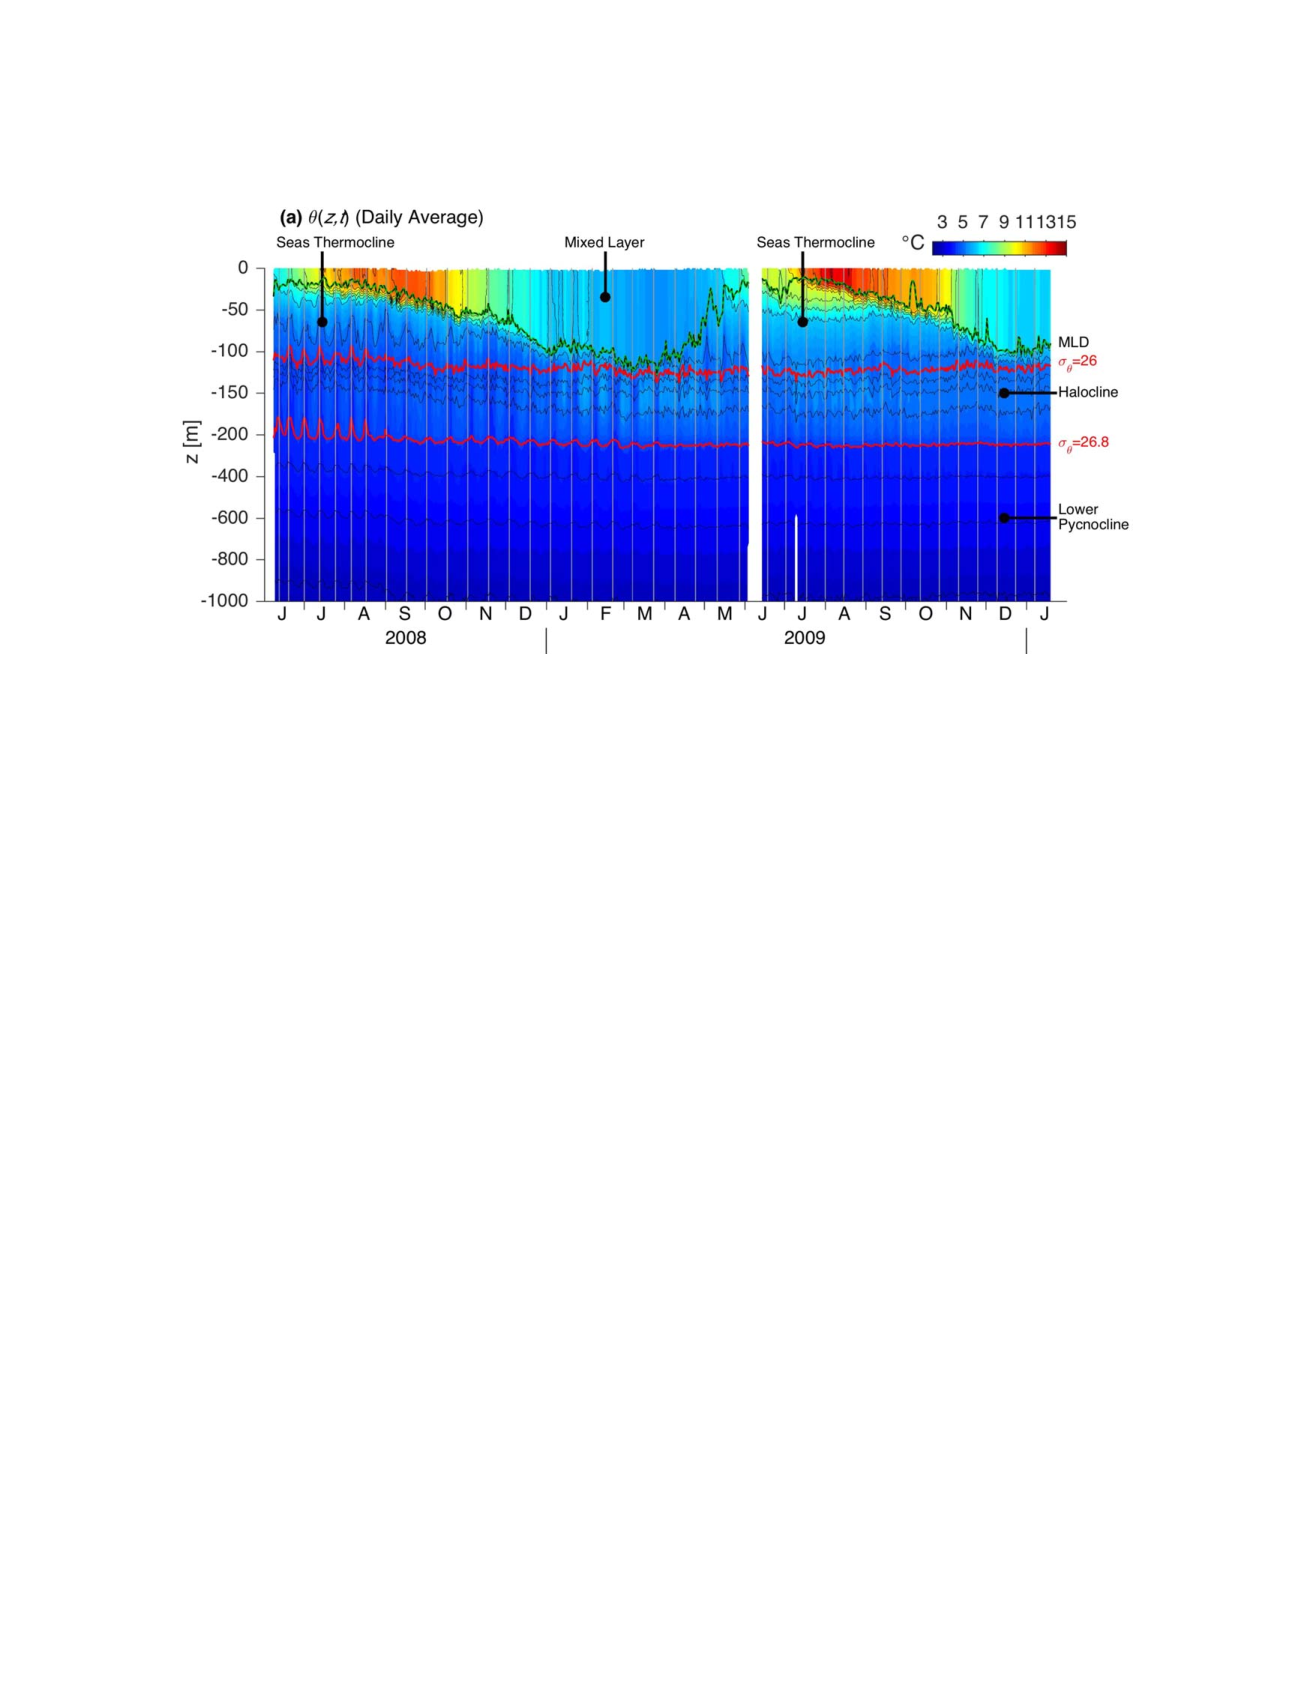
\includegraphics[]{figs/WaterMasses/PellandEtAlTheta}
  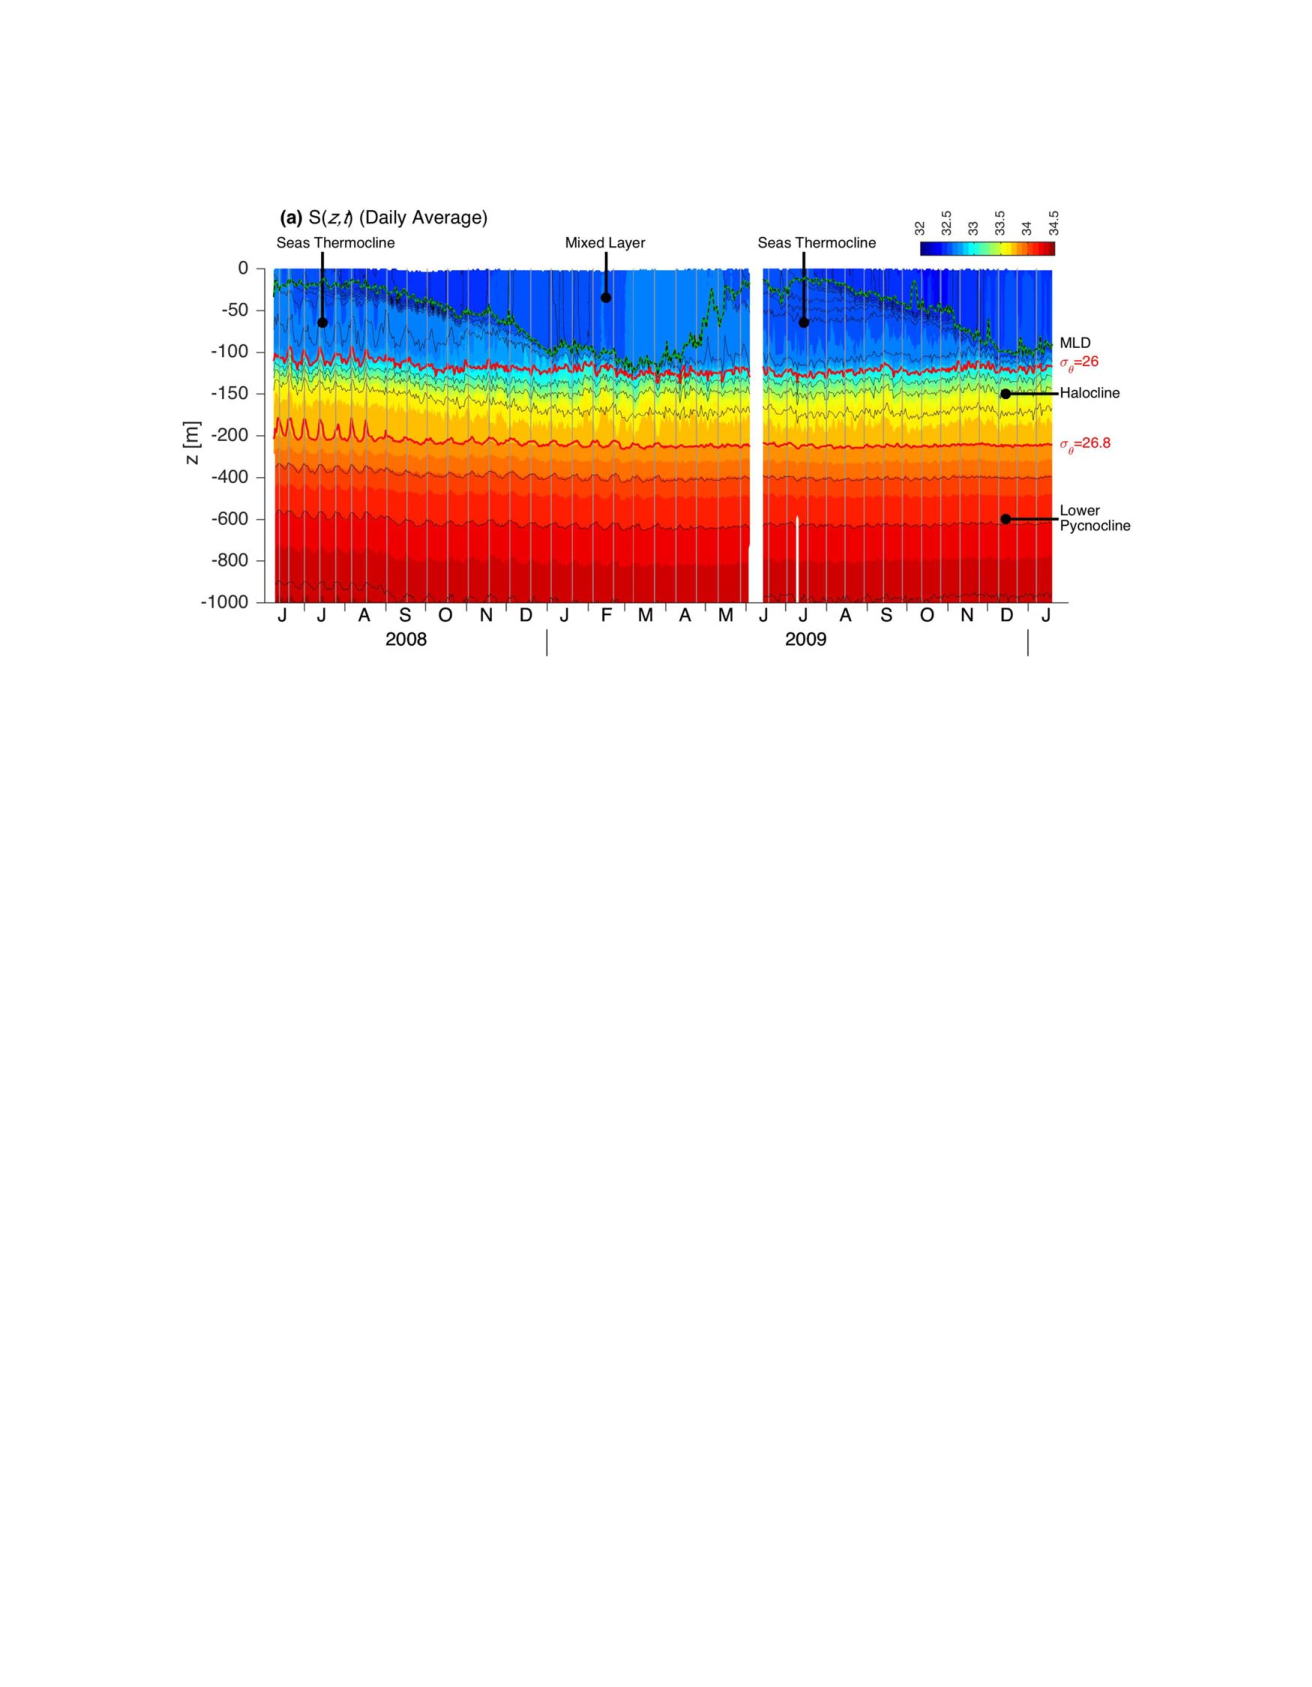
\includegraphics[]{figs/WaterMasses/PellandEtAlSal}
    \caption{Temperature and Salinity in the upper ocean over an annual cycle at Station Papa (Northeast Pacific Ocean: 50 N, 145 W) \citep{Pellandetal16}}
    \label{fig:PellandEtAl}  
\end{figure}

The mixed layer also evolves on a daily time scale, with warming in the dy and cooling at night, of course modified by the wind conditions (\fref{fig:MoumSmyth01Fig1}). In this example when the ocean is being warmed by the atmosphere, the mixed layer becomes very shallow  (\fref{fig:MoumSmyth01Fig1}B) and turbulence deeper in the water column is suppressed (\fref{fig:MoumSmyth01Fig1}C).  At night the water column cools and turbulence gets to deeper depths.

\begin{figure}[htp]
  \centering
  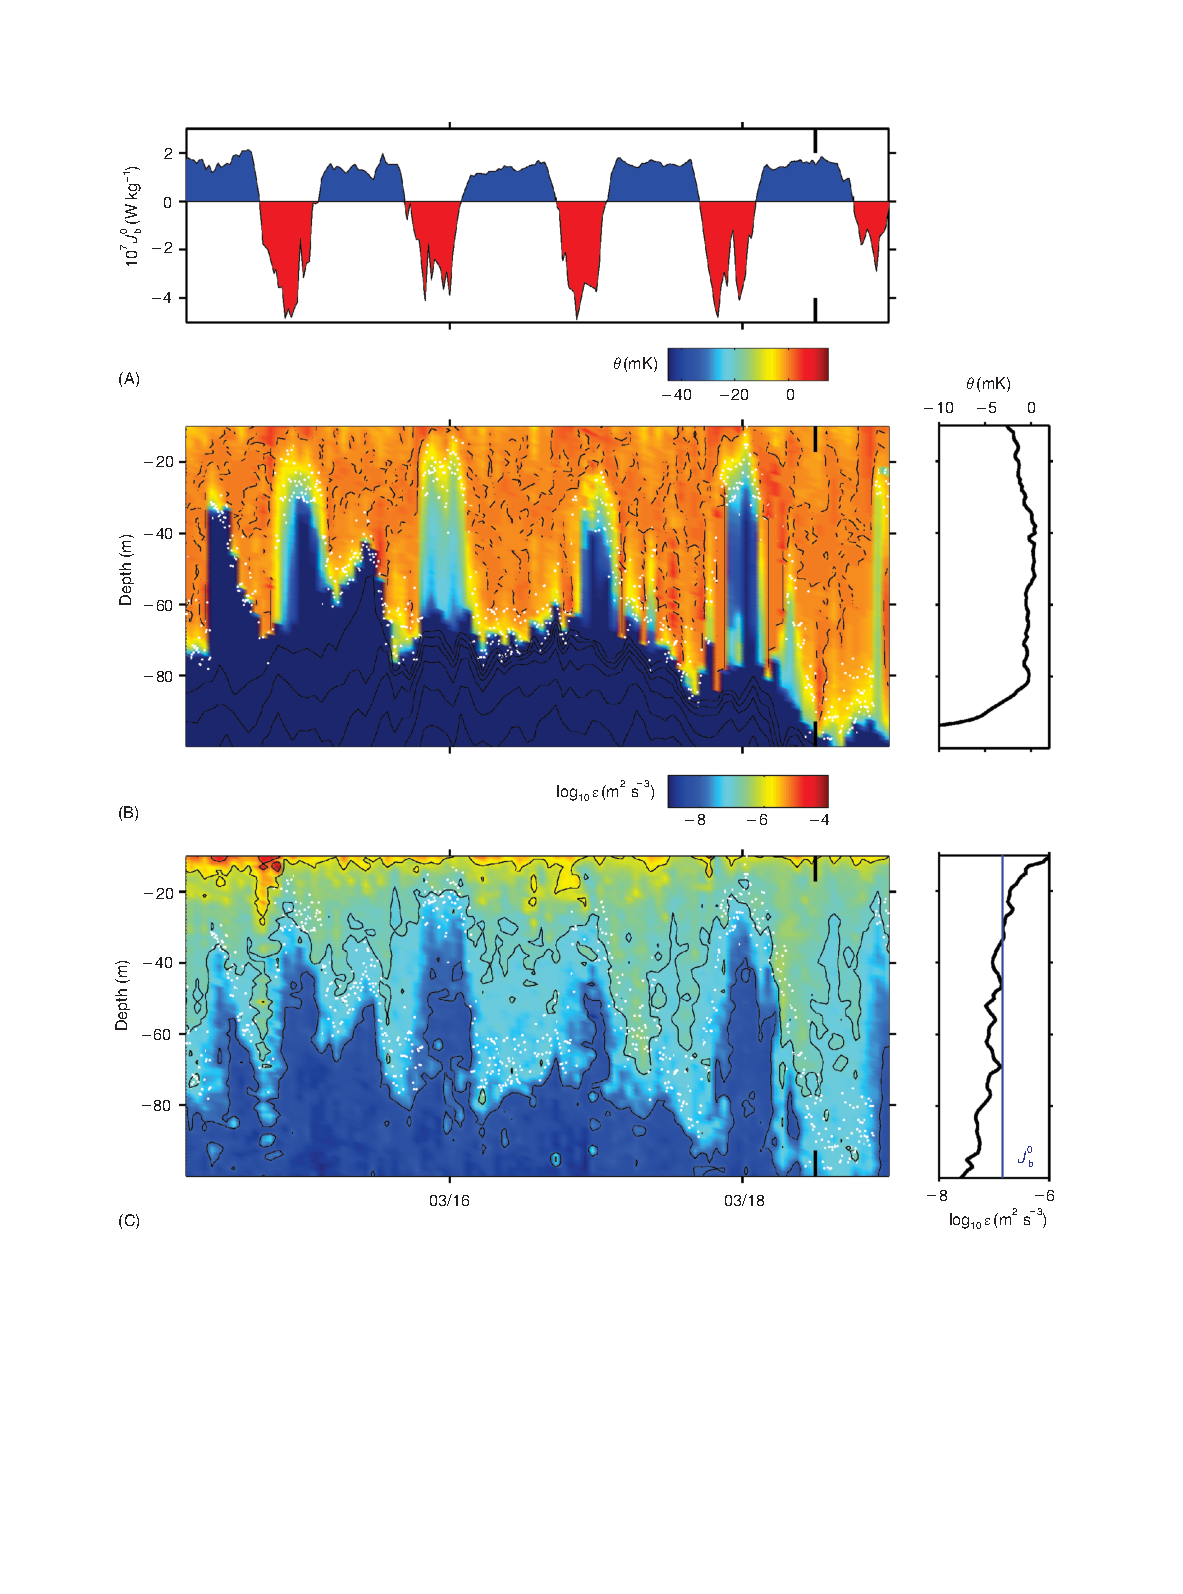
\includegraphics[]{figs/WaterMasses/MoumSmyth01Fig1}
    \caption{Mixing in the upper ocean in NE Pacific summer. A) heat flux, red being ocean heating, blue cooling. B) Temperature anomaly relative to depth-mean.  So this shows the vertical variation, but not the cooling and heating with time.  White dots indicate the base of the mixed layer.  C) Turbulence dissipation rate.  }
    \label{fig:MoumSmyth01Fig1}  
\end{figure}

Given the variety of forcings it is not surprising that the ocean mixed layer has a wide variety of depths through the worlds oceans (\fref{fig:Mixed_layer_depth}).  Depths are greatest in the winter, and reach quite great depths near the poles.  Depths also tend to be largest on the windward side of the basins, where there are the greatest heat fluxes.  

\begin{figure}[htp]
  \centering
  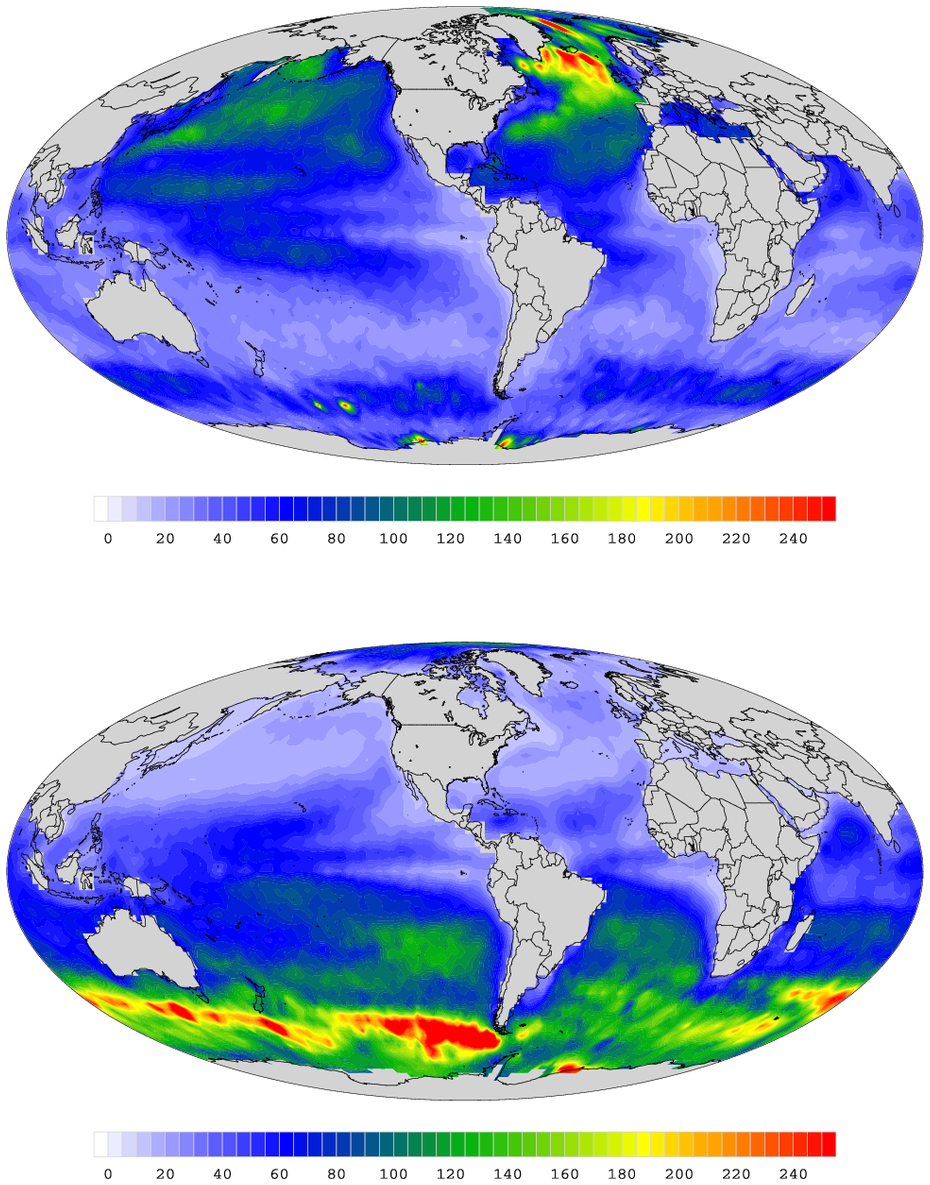
\includegraphics[width=3.5in]{WaterMasses/Mixed_layer_depth}
    \caption{Mixed layer depth in the boreal and austral winters. \protect\href{https://en.wikipedia.org/wiki/Mixed_layer#/media/File:Mixed_layer_depth.png}{from Wikipedia}}
    \label{fig:Mixed_layer_depth}  
\end{figure}

\begin{derivbox}[label={box:Restratification}]{Restratification of the mixed layer}
  \begin{center}
    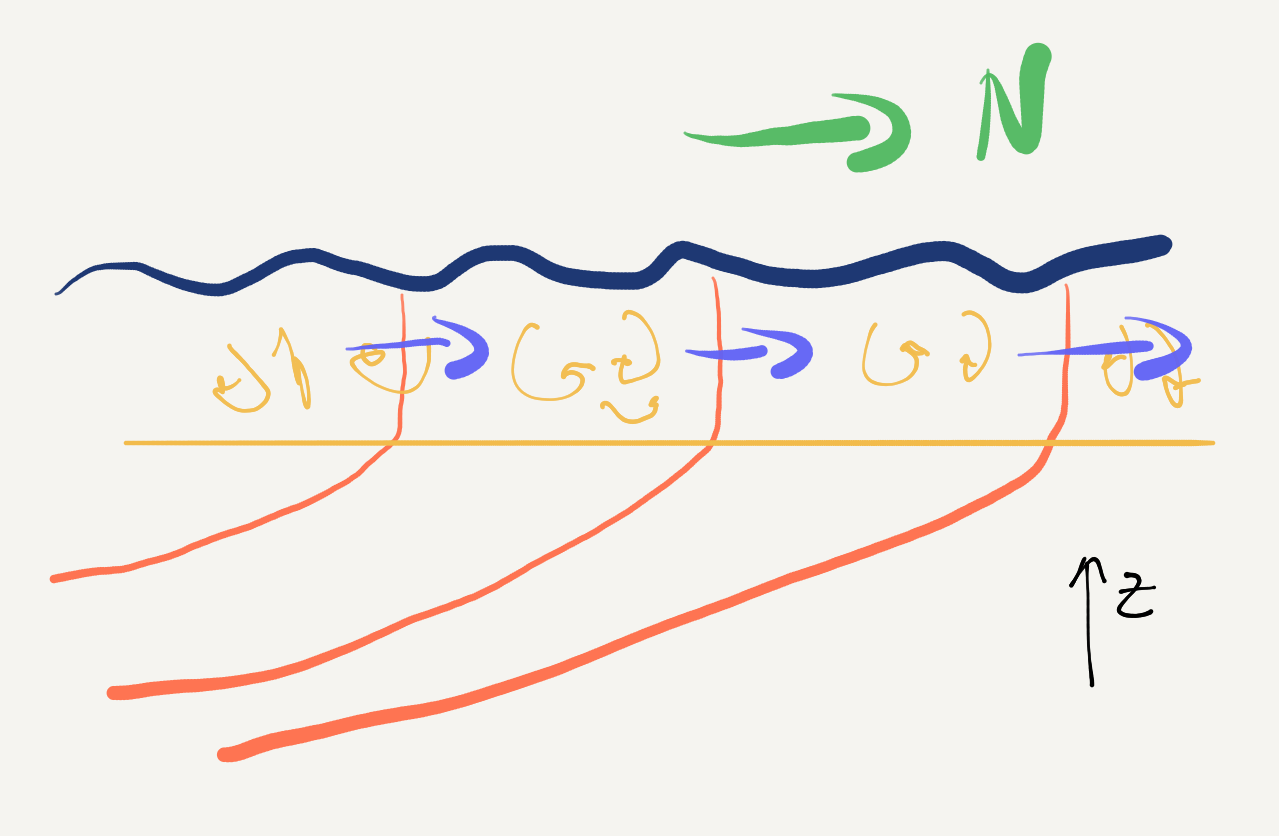
\includegraphics[width=3in]{figs/WaterMasses/SchemRestratfication}
  \end{center}
  A north-south section of the ocean in the northern hemisphere will tend to look like the schematic above.  If there were no mixing in the upper ocean, the orange ispycnals would tend to flatten, driving a flow to the North.  This happens all the time in the upper ocean where there is a warmer (lighter) mixed layer equatorward of a point.  Hence heat is being constantly fluxed poleward by this restratification, and if the mixed layer is to stay mixed, it must mix via turbulence and lose heat to the atmosphere.  So, when the north Pacific warms in the summer, it is not only the result of the local warming by the sun and lack of heat losses due to evaporation, but is also due to a northwards transport of heat by this restratification.  
\end{derivbox}

\section{Property-property plots: $\theta$-S plots}

As noted, the water masses tend to have particular characteristics.  Another useful tool for tracking water masses is to look at the data as property-property plots, and the most basic of these is a $\theta-S$ plot where potential temperature is plotted on the y axis, and salinity on the x-axis.  From this we can clearly see the differences between the different water masses from south to north.  At intermediate depths we can see the clear difference between warmer and fresher Pacific Intermediate Water at 34 psu and 7 degrees C, compared to the Antarctic Intermediate Water (34.25, 5 degrees C). 

Looking deeper, below 2000 m, we can see that the water in the Southern Ocean is substantially different than the water in the rest of the Pacific Ocean, with a large salty bulge at around (34.75 psu, 2 degrees C).  This distinct water is actually North Atlantic Deep Water that is found in the Southern Ocean, but does not make it into the rest of the Pacific Ocean.  The very densest water, at the bottom of the T-S curves, gets lighter both by warming and freshening.  

\begin{figure}[htp]
  \centering
  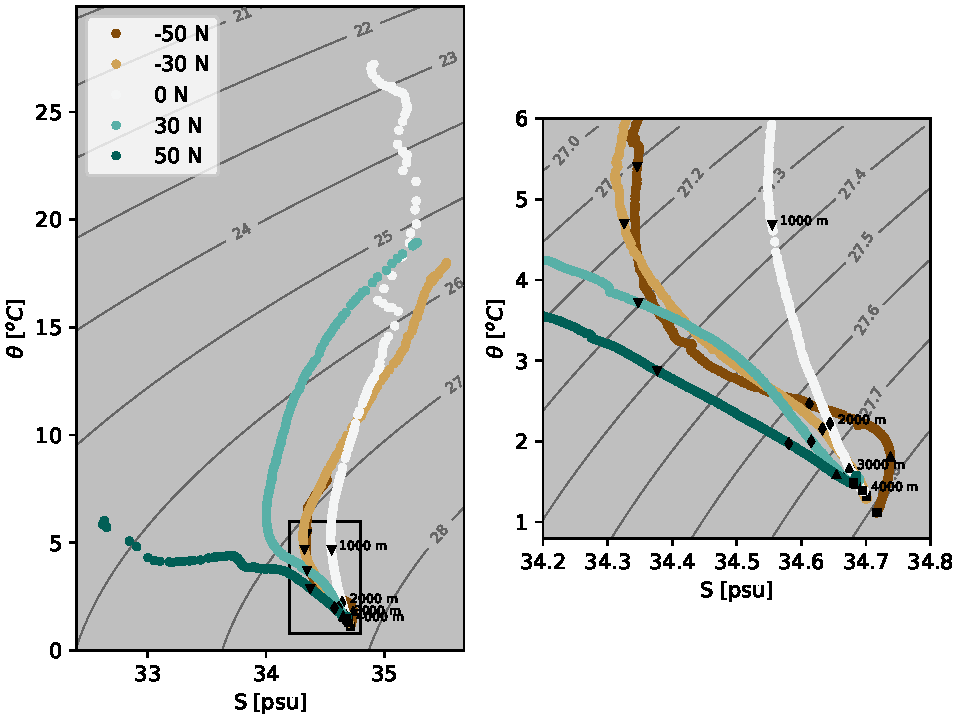
\includegraphics[]{WaterMasses/PacificExampleTS}
      \caption{Example T-S plots from along P16 in the Pacific, from the profiles shown in \fref{fig:ExamplePacificProfiles}.  The depth of the data are shown with symbols on each curve, and the right hand side is meant to emphasize the properties in the deepest 1000 m. The white line has the depths labeled.  Grey contours are potential density relative to the sea surface.}
    \label{fig:PacificExampleTS}  
\end{figure}

We can see how the properties vary smoothly with latitude by considering all the T-S curves along P16 (\fref{fig:P16TS}).  The cold and very fresh surface waters near the poles show up as large anomalies.  The anomalies are quickly eroded bust still show up as the intermediate water masses.  These intermediate water masses disappear, becoming more salty as the equator is approached.  

\begin{figure}[htp]
  \centering
  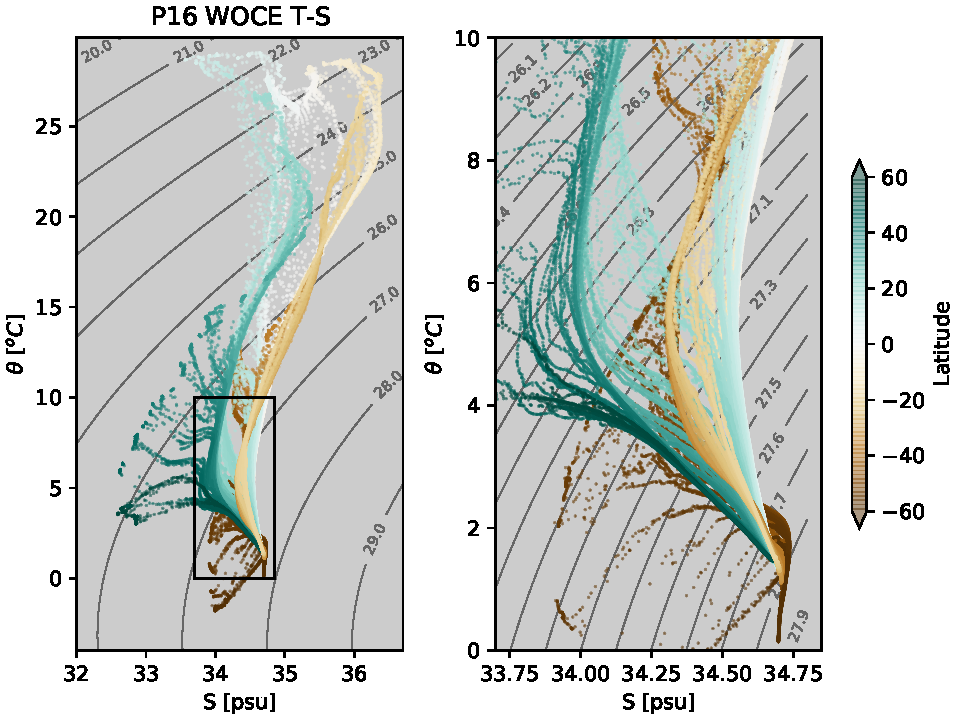
\includegraphics[width=3.5in]{WaterMasses/P16TS}
      \caption{WOCE $\theta-S$ properties along P16.  Data is color-coded by latitude.}
    \label{fig:P16TS}  
\end{figure}

The power of looking at T-S diagrams is that water should maintain its temperature and salinity properties away from the surface of the ocean, except via mixing between the water masses.  Mixing can be inferred from \emph{end members} which tend to mix along straight lines in T/S space.  For instance, if we mix equal parts water with salinity and temperature $S_1$ and $\theta_1$ with a second water mass $S_2, \theta_2$, then the mixture will have a new salinity $(S_1 + S_2) / 2$, and potential temperature $(\theta_1 + \theta_2)/2$ (\fref{fig:SketchTSMix}).  This new water mass lies on the line connecting the two water masses in space.  If there is more of one water mass is in the mixture, the point will still be along the line connecting the two water masses in T/S space, but it will be closer to the dominant water mass.

\begin{marginfigure}
  \centering
  \includegraphics[width=2.5in]{WaterMasses/SketchTSMix}
      \caption{Result of mixing two water masses in T/S space.  An equal mixture will lie midway on the line between the two water masses.  An unequal mixture will also be along the line.  }
    \label{fig:SketchTSMix}  
\end{marginfigure}


\begin{derivbox}[label={box:TSalongLine}]{Quick proof that mixture is along line between endpoints}
The line connecting $S_1,\theta_1$ and $S_2,\theta_2$ is given by 
\begin{equation}
    \theta = \frac{\theta_2 - \theta_1}{S_2 - S_1} \left(S-S_1 \right) + \theta_1
\end{equation}
If we then substitute $S=\frac{aS_1 + bS_2}{a+b}$ we get
\begin{eqnarray*}
    \theta & = & \frac{\theta_2 - \theta_1}{S_2 - S_1} \left( \frac{aS_1 + bS_2}{a+b}-S_1 \right) + \theta_1\\
    & = & \frac{\theta_2 - \theta_1}{S_2 - S_1} \left( \frac{-bS_1 + bS_2}{a+b}\right) + \theta_1\\
    & = & \frac{b\theta_2 - b \theta_1+ a\theta_1 + b\theta_1}{a+b}\\
    & = & \frac{a\theta_1 + b\theta_2}{a+b}     
\end{eqnarray*}
so $\frac{aS_1 + bS_2}{a+b}, \frac{a\theta_1 + b\theta_2}{a+b}$ lies along the line between the two water masses for any values of $a>0$ and $b>0$.  If either $a$ or $b$ are less than zero, the point lies beyond the two end point, which is not a possible situation for mixing.  
\end{derivbox}

The same principle applies if there are more water masses, though this becomes more complicated.  Usually, to start, the mixing is just between two water masses, and the newly mixed water falls along a T-S line; in \fref{fig:TSMixEvolve} the second row of plots shows what happens after a moderate amount of mixing between three water masses.  There are two T-S lines, and the data will follow a "V" shape.  As more mixing occurs, the original water masses start to be mixed way, until the final steady state of complete mixing is reached (\fref{fig:TSMixEvolve}, last row, step=9999).  Note that during this whole time the mixed product stays within the triangle defined by the three water masses we started with.  Indeed, unless there are surface processes, the T-S properties of any water parcel made up of these water masses \emph{must} fall within this envelope.  

\begin{figure}[htp]
  \centering
  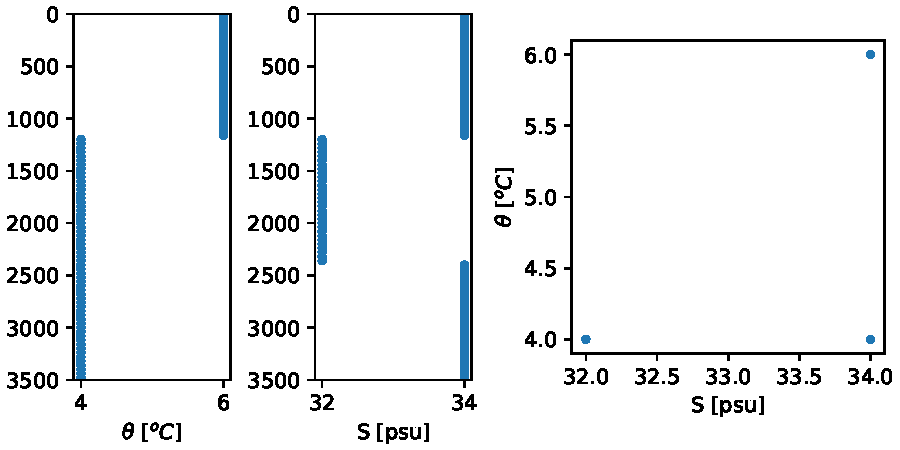
\includegraphics[width=3in]{WaterMasses/TSMixInitial}
  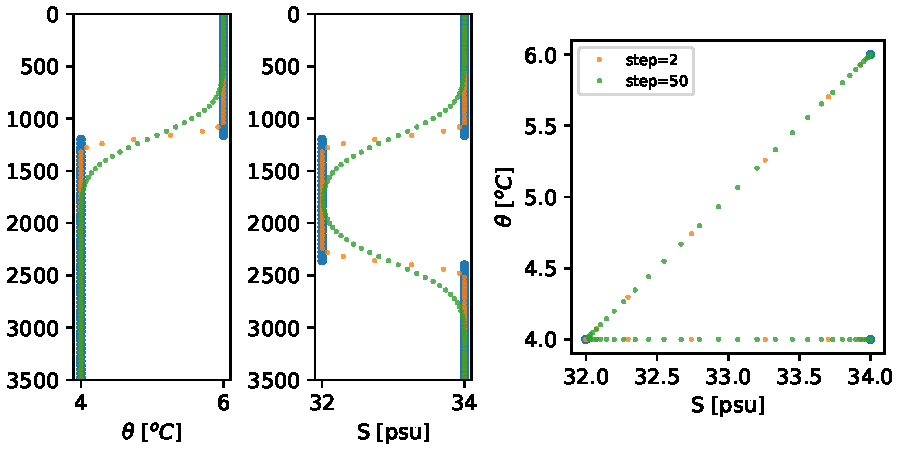
\includegraphics[width=3in]{WaterMasses/TSMixMiddle}
    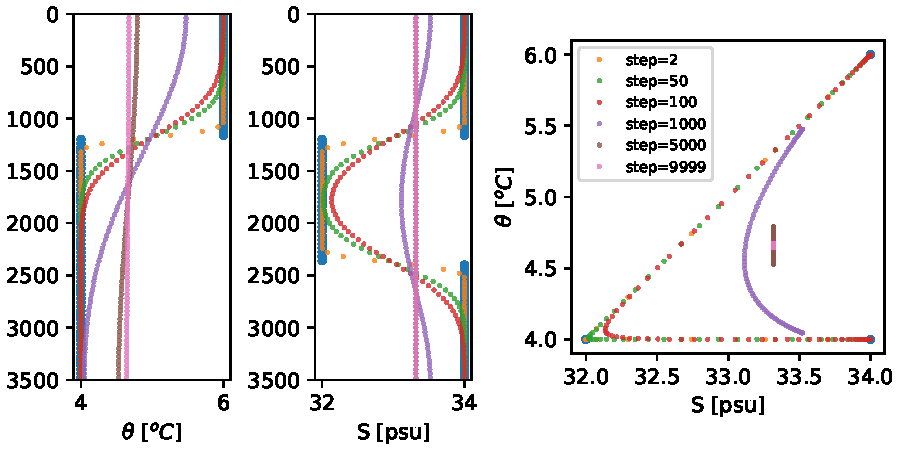
\includegraphics[width=3in]{WaterMasses/TSMixFinal}
      \caption{Result of mixing three water masses that are originally well mixed.  The first row is the initial state. The second row is after some mixing has occurred, but all three water masses still exist.  The last row is what happens after a long time.  Eventually the temperature and salinity are well-mixed and all the points coalesce to a dot in T-S space. }
    \label{fig:TSMixEvolve}  
\end{figure}

We can then look at the WOCE data again, considering the origin of the water masses in the southern hemisphere (\fref{fig:P16TSSouthern}).  If there were no North Atlantic Deep Water, there would be no kink in the T-S curves between $\gamma_N = 27.7$ and $\gamma_N=27.8$.  By the time we get to the equator (white line), the T/S curve looks a lot like the schematic shown in \fref{fig:TSMixEvolve}, where it curves between the bottom water and the surface towards the AAIW.  

\begin{figure}[htp]
  \centering
  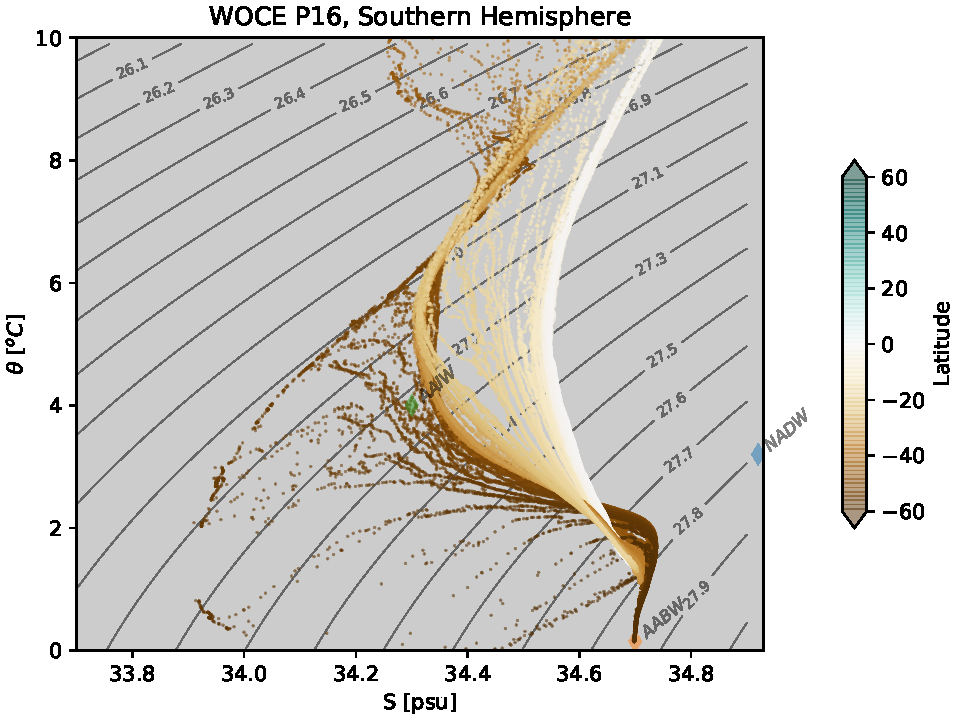
\includegraphics{figs/WaterMasses/P16TSSouthern}
      \caption{T/S diagram of the southern hemisphere Pacific, with core water masses indicated}
    \label{fig:P16TSSouthern}  
\end{figure}

\section{Summary}

\begin{itemize}
    \item The water properties in the ocean are largely set at the surface by heat and freshwater fluxes
    \item There are few locations where water is able to sink away from the surface, namely:
        \begin{enumerate}
            \item the subpolar gyres: Intermediate waters
            \item marginal seas: i.e. Mediterranean and Red Seas
            \item high latitudes (also often marginal seas): Antarctic Bottom Water, and North Atlantic Deep Water.
        \end{enumerate}
    \item Subsurface waters can be traced over great areas in the worlds oceans with identifiable \emph{core waters}.
    \item T-S properties are mixed along \emph{mixing lines}. 
\end{itemize}

We will discuss in the next chapter where the deep waters arise and why they circulate as they do.  

%%% Local Variables:
%%% mode: latex
%%% TeX-master: t
%%% End:
